\chapter{The Quantum Harmonic Oscillator}

Susskind opens this lecture by calling it the final class in quantum mechanics and then immediately taking that back: quantum mechanics will return when the course reaches quantum field theory. Still, as he says, the harmonic oscillator is one of the last indispensable pieces of the elementary subject. It is worth doing with some care, because it is not merely a spring with a mass attached to it. The same mathematics reappears whenever a system has a stable equilibrium and we disturb it only slightly. The lecture unfolds in that order: broad motivation first, then the classical oscillator, then quantization, then the question of why only special energies are allowed, and finally the algebra that generates the whole spectrum.

\paragraph{Credit.} These notes follow Leonard Susskind's lecture closely. The preserved blackboard frames are kept as documentary support for the derivation, with credit to Leonard Susskind, LazyingArt LLC, and Video2Book.

\section{Why This System Matters}

The first task is not to write down an equation, but to understand why this system deserves attention at all. The harmonic oscillator is, in Susskind's words, basically a particle moving on a line under the influence of a restoring force. A spring is the obvious example, but the lecture immediately broadens the point. A point on a passing wave oscillates. A sound wave oscillates. Molecules vibrate about equilibrium configurations. In fact, almost any system with a stable equilibrium behaves this way when it is disturbed only a little.

That is the real reason for quantizing the oscillator. There is no practical urgency in quantizing a visible laboratory spring with a heavy mass hanging from it; for such a system the quantum corrections are utterly negligible. But the same mathematics does apply to molecular motion and to many other genuinely microscopic systems. We therefore use the spring as a model, not because it is the only oscillator, but because it is the cleanest entry point.

There is also a more precise way to state the generality. Suppose a one-dimensional potential has a stable minimum at \(x_{0}\). Then near that minimum we may expand
\begin{equation}
V(x)\approx V(x_{0})+\frac{1}{2}V''(x_{0})(x-x_{0})^{2}.
\end{equation}
A local minimum therefore looks, to quadratic order, like a parabola. Near a stable point, the world becomes harmonic.

\section{Classical Oscillator From Spring Sketch to Equation of Motion}

The lecture begins concretely with a weight hanging from a spring. Gravity pulls downward, the spring pulls upward, and there is an equilibrium position at which the two balance. Once that equilibrium has been found, the sensible coordinate is not the absolute height but the displacement from equilibrium. Susskind chooses to call that displacement \(x\), even though in the picture it is drawn vertically.

\begin{figure}[ht]
\centering

\includegraphics[width=0.72\textwidth]{lecture_10_figure_02.png}
\caption{Spring-mass oscillator and the quadratic Lagrangian term.}
\label{fig:ho_classical_board_refined}
\end{figure}

\begin{figure}[ht]
\centering
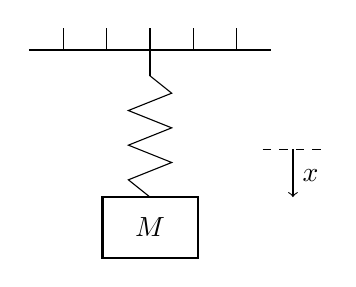
\begin{tikzpicture}[scale=1.1]
\draw[thick] (-1.4,2.6)--(1.4,2.6);
\draw (-1.0,2.6)--(-1.0,2.85);
\draw (-0.5,2.6)--(-0.5,2.85);
\draw (0.0,2.6)--(0.0,2.85);
\draw (0.5,2.6)--(0.5,2.85);
\draw (1.0,2.6)--(1.0,2.85);
\draw (0,2.6)--(0,2.3);
\draw (0,2.3)--(0.25,2.1)--(-0.25,1.9)--(0.25,1.7)--(-0.25,1.5)--(0.25,1.3)--(-0.25,1.1)--(0,0.9);
\draw[thick] (-0.55,0.2) rectangle (0.55,0.9);
\node at (0,0.55) {\(M\)};
\draw[dashed] (1.3,1.45)--(2.0,1.45);
\draw[->] (1.65,1.45)--(1.65,0.9);
\node[right] at (1.65,1.15) {\(x\)};
\end{tikzpicture}
\caption{A clean redraw of the spring-mass sketch used in the classical setup.}
\label{fig:ho_classical_tikz_refined}
\end{figure}

Once the equilibrium position has been absorbed into the definition of \(x\), gravity disappears from the local dynamics. The only remaining ingredients are kinetic energy and the restoring potential. Susskind then makes a second simplification: he absorbs the mass into the coordinate. If the original displacement is \(x_{\mathrm{old}}\), then one may define
\begin{equation}
y=\sqrt{m}\,x_{\mathrm{old}},
\qquad
\dot y^{\,2}=m\,\dot x_{\mathrm{old}}^{\,2}.
\end{equation}
After exhibiting this rescaling explicitly, he simply renames the new coordinate \(x\). The mass has thus been scaled out, and the spring constant is renamed \(\omega^{2}\). With those choices the Lagrangian becomes
\begin{equation}
L=\frac{1}{2}\dot x^{2}-\frac{1}{2}\omega^{2}x^{2}.
\label{eq:ho_lagrangian}
\end{equation}

The potential energy must be proportional to \(x^{2}\), not to \(x\), because the energy should increase whether the system is displaced to the right or to the left. That is the local signature of a stable equilibrium. The canonical momentum is
\begin{equation}
p=\frac{\partial L}{\partial \dot x}=\dot x.
\end{equation}
Applying the Euler--Lagrange equation,
\begin{equation}
\frac{d}{dt}\frac{\partial L}{\partial \dot x}-\frac{\partial L}{\partial x}=0,
\end{equation}
we find
\begin{equation}
\ddot x=-\omega^{2}x.
\label{eq:ho_classical_eom}
\end{equation}
The minus sign is the restoring sign. If \(x\) is positive, the force points back toward the origin; if \(x\) is negative, it again points back toward the origin.

The general classical solution is therefore
\begin{equation}
x(t)=a\cos\omega t+b\sin\omega t.
\end{equation}
So much for the classical oscillator. The point of doing this first is that the quantum system will inherit the same Hamiltonian structure.

\section{Quantization Setup: States, Operators, and the Hamiltonian}

To go from the classical oscillator to the quantum oscillator, Susskind insists that we proceed in the usual order. First we specify the space of states. Only then do we construct the Hamiltonian operator.

For a particle moving on a line, the state space is the space of wave functions \(\psi(x)\). The probability density is
\begin{equation}
|\psi(x)|^{2}=\psi^{*}(x)\psi(x).
\end{equation}
In the \(x\)-representation the position operator acts by multiplication:
\begin{equation}
\hat x\,\psi(x)=x\,\psi(x).
\end{equation}
The momentum operator, temporarily setting \(\hbar=1\), acts as
\begin{equation}
\hat p\,\psi(x)=-i\frac{\partial \psi}{\partial x}.
\end{equation}
The lecture pauses here to emphasize that \(x\) and \(p\) are Hermitian operators acting on the vector space of wave functions.

On the classical side, the Hamiltonian comes from the Lagrangian in the standard way:
\begin{align}
H
&=
p\dot x-L \\
&=
\frac{1}{2}\dot x^{2}+\frac{1}{2}\omega^{2}x^{2} \\
&=
\frac{1}{2}p^{2}+\frac{1}{2}\omega^{2}x^{2}.
\label{eq:ho_classical_H}
\end{align}
This three-line progression is visible on the board and is worth preserving because it is exactly how the lecture moves.

\begin{figure}[ht]
\centering

\includegraphics[width=0.72\textwidth]{lecture_10_figure_03.png}
\caption{Hamiltonian rewritten as an operator on the wave function.}
\label{fig:ho_hamiltonian_board_refined}
\end{figure}

Once we quantize, the Hamiltonian acts on a wave function as
\begin{align}
H\psi(x)
&=
\frac{1}{2}\hat p^{\,2}\psi(x)+\frac{1}{2}\omega^{2}x^{2}\psi(x) \\
&=
-\frac{1}{2}\frac{\partial^{2}\psi}{\partial x^{2}}
+\frac{1}{2}\omega^{2}x^{2}\psi(x).
\label{eq:ho_operator_action}
\end{align}
The bottom line of the board uses a quick correspondence between ket notation and the coordinate representation; here we normalize it into the cleaner operator notation \eqref{eq:ho_operator_action}.

\section{Two Uses of the Hamiltonian and the Energy Eigenvalue Problem}

At this point the lecture makes an important distinction. The Hamiltonian has two jobs. One is to govern the time evolution of the state. The other is to determine the allowed energy levels.

The time-dependent Schr\"odinger equation is
\begin{equation}
i\frac{\partial \psi(x,t)}{\partial t}=H\psi(x,t).
\label{eq:ho_tdse}
\end{equation}
Substituting \eqref{eq:ho_operator_action}, we obtain
\begin{equation}
i\frac{\partial \psi}{\partial t}
=
-\frac{1}{2}\frac{\partial^{2}\psi}{\partial x^{2}}
+\frac{1}{2}\omega^{2}x^{2}\psi.
\end{equation}
Because of the factor of \(i\), even a real wave function at \(t=0\) will generically acquire an imaginary part as time evolves. So the wave function must be allowed to be complex.

Susskind briefly notes that one could solve this dynamics directly, for example by updating the wave function in small time steps. At the schematic level one would write
\begin{equation}
\psi(x,t+\delta t)\approx \psi(x,t)-i\,\delta t\,H\psi(x,t).
\end{equation}
That is the dynamical problem. But he then narrows the focus quite deliberately: let us instead look for the energy eigenvectors themselves.

Those satisfy
\begin{equation}
H\psi_{E}(x)=E\,\psi_{E}(x),
\end{equation}
which in explicit form becomes
\begin{equation}
-\frac{1}{2}\psi_{E}''(x)+\frac{1}{2}\omega^{2}x^{2}\psi_{E}(x)=E\,\psi_{E}(x).
\label{eq:ho_tise_refined}
\end{equation}
This equation does two things at once. It is an equation for the wave function \(\psi_{E}(x)\), but it also selects the allowed values of \(E\).

Why should not every value of \(E\) be allowed? The lecture answers this in the most direct way possible. Equation \eqref{eq:ho_tise_refined} is a second-order differential equation, so for a generic energy there are two linearly independent solutions. At large \(|x|\), the quadratic potential dominates, and at the rough level needed here the solutions behave like Gaussian-type exponentials,
\begin{equation}
\psi(x)\sim \exp\!\left(-\frac{\omega x^{2}}{2}\right)
\quad \text{or} \quad
\psi(x)\sim \exp\!\left(+\frac{\omega x^{2}}{2}\right),
\qquad |x|\to\infty,
\end{equation}
up to subleading factors.

The lecture is careful not to leave this as a slogan. The generic second-order situation is actually worse than merely having one good global solution and one bad global solution. More typically, a solution that decays in one direction blows up in the other, and vice versa. Only for very special energies does a single solution decay in both directions. Those are the energy eigenvalues.

The physical criterion is square-integrability:
\begin{equation}
\int_{-\infty}^{\infty}|\psi(x)|^{2}\,dx=1.
\label{eq:normalization_condition}
\end{equation}
A wave function that blows up exponentially pushes all its probability out to infinity, and in a confining potential that also means infinite potential energy. So the discrete spectrum is not being imposed by hand; it emerges from the demand that the state be admissible.

\section{Ground-State Guess and Zero-Point Energy}

Having explained why only certain energies can work, the lecture next looks for one concrete solution. This is the first real payoff. Susskind guesses a Gaussian concentrated near the origin. In the live lecture there is a moment of hesitation about the factor of \(1/2\) in the exponent; the cleaned result is
\begin{equation}
\psi_{0}(x)\propto e^{-\frac{\omega}{2}x^{2}}.
\end{equation}
We leave the normalization constant aside for now, exactly as the lecture does.

\begin{figure}[ht]
\centering

\includegraphics[width=0.82\textwidth]{lecture_10_figure_04.png}
\caption{Gaussian trial state checked as an energy eigenvector.}
\label{fig:ho_gaussian_board_refined}
\end{figure}

The blackboard calculation is partly hard to read in the middle, but its logical structure is clear: differentiate, differentiate again, substitute into the Hamiltonian, and watch the \(x^{2}\) terms cancel. In cleaned notation,
\begin{equation}
\psi_{0}'(x)=-\omega x\,\psi_{0}(x),
\end{equation}
and then
\begin{equation}
\psi_{0}''(x)=(-\omega+\omega^{2}x^{2})\psi_{0}(x).
\end{equation}
Now act with the Hamiltonian:
\begin{align}
H\psi_{0}
&=
-\frac{1}{2}\psi_{0}''+\frac{1}{2}\omega^{2}x^{2}\psi_{0} \\
&=
-\frac{1}{2}(-\omega+\omega^{2}x^{2})\psi_{0}
+\frac{1}{2}\omega^{2}x^{2}\psi_{0} \\
&=
\left(
\frac{\omega}{2}
-\frac{\omega^{2}x^{2}}{2}
+\frac{\omega^{2}x^{2}}{2}
\right)\psi_{0} \\
&=
\frac{\omega}{2}\psi_{0}.
\end{align}
Thus the Gaussian really is an eigenfunction, and its energy is
\begin{equation}
E_{0}=\frac{\omega}{2}.
\end{equation}
This is the ground-state energy. Restoring \(\hbar\) at the end gives
\begin{equation}
E_{0}=\frac{\hbar\omega}{2}.
\end{equation}
The lecture then pauses to underline the point: classically the minimum energy would be zero, but quantum mechanically the lowest state already has nonzero energy.

\subsection{Question \& Answer}

\paragraph{Why is there no zero-energy state?}

This is the natural conceptual obstacle raised by the lecture, and it is answered in three mutually reinforcing ways.

\begin{figure}[ht]
\centering

\includegraphics[width=0.58\textwidth]{lecture_10_figure_05.png}
\caption{Harmonic-oscillator Schr\"odinger equation during the \(\psi=1\) discussion.}
\label{fig:ho_zero_energy_board_refined}
\end{figure}

The equation under discussion is still
\begin{equation}
-\frac{1}{2}\psi''(x)+\frac{1}{2}\omega^{2}x^{2}\psi(x)=E\psi(x).
\end{equation}

\begin{enumerate}
\item The first answer is the uncertainty principle. Classically we would minimize the positive-definite Hamiltonian
\begin{equation}
H=\frac{1}{2}p^{2}+\frac{1}{2}\omega^{2}x^{2}
\end{equation}
by setting both \(x\) and \(p\) equal to zero. Quantum mechanically that is too much to ask. We can compromise, but we cannot make both vanish sharply. Therefore the lowest possible energy cannot be zero.

\item The second answer is the explicit test \(\psi(x)=1\). A constant wave function is indeed a zero-momentum state, because the derivative term vanishes on it. But it does not solve the eigenvalue equation:
\begin{equation}
H(1)=\frac{1}{2}\omega^{2}x^{2}\neq 0.
\end{equation}
So \(\psi=1\) kills the kinetic term but leaves the potential term untouched. It does not represent \(x=0\); it only represents zero momentum.

\item The third answer is the asymptotic one. If we set \(E=0\), we obtain
\begin{equation}
-\frac{1}{2}\psi''+\frac{1}{2}\omega^{2}x^{2}\psi=0.
\end{equation}
This equation does have formal solutions, but none of them is acceptable. One may tune initial conditions so that the solution decays in one direction, but then it blows up in the other. Typically it blows up in both directions. So \(E=0\) is excluded at the level of normalizable states.
\end{enumerate}

The lecture ends this exchange by stating the admissibility condition plainly: the state vectors of a properly defined quantum system must be normalizable. That can be posed as an axiom, but the lecture also offers the more satisfying physical explanation: otherwise all the probability would sit infinitely far away.

\section{Ladder Operators and the Algebraic Reformulation}

After the break, the method changes. Up to this point the discussion has been in the language of differential equations. Now the lecture introduces the special algebraic trick that makes the harmonic oscillator soluble in a completely different way.

Susskind begins with the unnormalized operators
\begin{equation}
b_{-}=p-i\omega x,
\qquad
b_{+}=p+i\omega x.
\end{equation}
The first reason for writing them is the elementary identity \(a^{2}+b^{2}=(a+ib)(a-ib)\). Classically one would simply rewrite the Hamiltonian as a product. Quantum mechanically the same manipulation is nearly right, but not quite right, because \(x\) and \(p\) do not commute.

\begin{figure}[ht]
\centering

\includegraphics[width=0.74\textwidth]{lecture_10_figure_06.png}
\caption{Hamiltonian in ladder-operator form.}
\label{fig:ho_ladder_board_refined}
\end{figure}

The live lecture contains some hesitation over signs and naming. The safest way to stabilize the notation is to demand that the operator with the minus sign annihilate the ground state; that is the clue Susskind himself uses. With \([x,p]=i\) and \(\hbar=1\), we compute
\begin{align}
b_{+}b_{-}
&=
(p+i\omega x)(p-i\omega x) \\
&=
p^{2}+\omega^{2}x^{2}+i\omega(xp-px) \\
&=
p^{2}+\omega^{2}x^{2}-\omega.
\end{align}
So the Hamiltonian may be written as
\begin{equation}
H=\frac{1}{2}(p^{2}+\omega^{2}x^{2})
=
\frac{1}{2}b_{+}b_{-}+\frac{\omega}{2}.
\label{eq:ho_b_factorization}
\end{equation}
The additional constant is precisely the zero-point energy already found by the Gaussian calculation. The lecture insists on this point: adding an ordinary number to an operator shifts all eigenvalues by the same amount and does nothing more mysterious than that.

Next we compute the commutator:
\begin{align}
[b_{-},b_{+}]
&=
[p-i\omega x,\,p+i\omega x] \\
&=
2\omega.
\end{align}
It is then convenient to divide by \(\sqrt{2\omega}\) and introduce the cleaned operators
\begin{equation}
a=\frac{1}{\sqrt{2\omega}}\,b_{-}
=\frac{1}{\sqrt{2\omega}}(p-i\omega x),
\qquad
a^{\dagger}=\frac{1}{\sqrt{2\omega}}\,b_{+}
=\frac{1}{\sqrt{2\omega}}(p+i\omega x).
\end{equation}
By construction,
\begin{equation}
[a,a^{\dagger}]=1.
\end{equation}
Equation \eqref{eq:ho_b_factorization} becomes
\begin{equation}
H=\omega\left(a^{\dagger}a+\frac{1}{2}\right).
\label{eq:ho_ladder_H_refined}
\end{equation}

Now the ground state reveals itself algebraically. Since
\begin{equation}
a=\frac{1}{\sqrt{2\omega}}(p-i\omega x),
\end{equation}
we find
\begin{align}
a\,\psi_{0}
&=
\frac{1}{\sqrt{2\omega}}
\left(
-i\frac{d}{dx}-i\omega x
\right)e^{-\omega x^{2}/2} \\
&=
-\frac{i}{\sqrt{2\omega}}
\left(
\frac{d}{dx}+\omega x
\right)e^{-\omega x^{2}/2} \\
&=
0,
\end{align}
because
\(
\frac{d}{dx}e^{-\omega x^{2}/2}=-\omega x e^{-\omega x^{2}/2}.
\)
So the operator \(a\) annihilates the ground state. That is why it is the lowering operator.

\section{Spectrum, Excited States, and What the Wave Functions Mean}

Once the Hamiltonian has the form \eqref{eq:ho_ladder_H_refined}, the problem becomes algebraic. Let
\begin{equation}
N=a^{\dagger}a
\end{equation}
and suppose
\begin{equation}
N|n\rangle=n|n\rangle.
\end{equation}
Then
\begin{align}
N(a^{\dagger}|n\rangle)
&=
a^{\dagger}a\,a^{\dagger}|n\rangle \\
&=
a^{\dagger}(aa^{\dagger})|n\rangle \\
&=
a^{\dagger}(a^{\dagger}a+1)|n\rangle \\
&=
(n+1)a^{\dagger}|n\rangle.
\end{align}
So \(a^{\dagger}\) raises the eigenvalue of \(N\) by one. Similarly, \(a\) lowers it by one until the ground state is reached, at which point it gives zero. The whole spectrum is therefore
\begin{equation}
E_{n}=\omega\left(n+\frac{1}{2}\right),
\qquad n=0,1,2,\dots
\end{equation}
or, with \(\hbar\) restored,
\begin{equation}
E_{n}=\hbar\omega\left(n+\frac{1}{2}\right).
\end{equation}
This is exactly the equally spaced ladder that the lecture is aiming toward.

The first excited wave function may be found directly by acting once with the raising operator:
\begin{align}
\psi_{1}(x)
&\propto
a^{\dagger}\psi_{0}(x) \\
&=
\frac{1}{\sqrt{2\omega}}
\left(
-i\frac{d}{dx}+i\omega x
\right)e^{-\omega x^{2}/2} \\
&\propto
x\,e^{-\omega x^{2}/2}.
\end{align}
Up to an overall constant and phase, the first excited state is the Gaussian multiplied by \(x\). It has one node at the origin.

This is the pattern the lecture wants us to notice. Repeated action of \(a^{\dagger}\) produces a Gaussian multiplied by higher and higher polynomials:
\begin{equation}
\psi_{n}(x)=P_{n}(x)e^{-\omega x^{2}/2},
\end{equation}
where \(P_{n}(x)\) is a degree-\(n\) polynomial. The lecture does not turn this into a full Hermite-polynomial discussion, and it is better not to overstate what was actually motivated. The important qualitative points are these:
\begin{itemize}
\item each new excitation introduces one more node;
\item the parity alternates from symmetric to antisymmetric and back again;
\item the wave function oscillates more rapidly as the energy increases, indicating larger momentum content;
\item the wave function also spreads farther from the origin, reflecting larger excursions in position.
\end{itemize}

The lecture adds one further observation. An equally spaced spectrum is not by itself enough to characterize the harmonic oscillator. One can invent other operators with equally spaced eigenvalues, but they may extend upward and downward without bound. What makes the oscillator special, within the scope of this lecture, is the combination of equal spacing and a spectrum bounded from below.

\subsection{Question \& Answer}

\paragraph{What does a quantum harmonic oscillator look like?}

Late in the lecture, a student asks what such a system physically looks like. Susskind's answer is that this is not quite the right question. A quantum system is not something we simply stare at or photograph without disturbing it. The more meaningful question is what its probability distributions look like.

For the ground state, the probability density is Gaussian. It is concentrated near the minimum and has a width controlled by \(\omega\). The larger \(\omega\) is, the tighter the restoring force, and the narrower the wave function becomes. This is exactly the interpretation Susskind gives in words: a stiffer spring holds the system more tightly to the origin.

Above the ground state, the probability density develops nodes. There are points at which the probability is exactly zero. The lecture treats this as one of the distinctly quantum features of the oscillator: the particle is still, in an appropriate sense, an oscillator, but the wave function can have exact zeros produced by interference.

This returns us to the broad motivation with which the lecture began. A quantum harmonic oscillator is not a tiny visible spring. It is the local quantum description of motion near a stable minimum. A diatomic molecule is a good example. More generally, whenever a system has a stable configuration and we study small deviations from it, the potential near the minimum is approximately quadratic, and the quantized motion is approximately that of the harmonic oscillator.

\section{Summary}

The lecture develops the harmonic oscillator in the same order in which one would discover it if one were being careful. We begin with a concrete spring and a classical Lagrangian, shift the coordinate to equilibrium, scale out the mass, and arrive at
\(
\ddot x=-\omega^{2}x.
\)
We then quantize the system by specifying the space of states, representing \(x\) and \(p\) as operators, and writing the Schr\"odinger equation. The discrete spectrum appears because acceptable wave functions must be normalizable.

The first explicit payoff is the Gaussian ground state
\(
\psi_{0}(x)\propto e^{-\omega x^{2}/2},
\)
with zero-point energy
\(
E_{0}=\hbar\omega/2.
\)
The second is the algebraic reformulation
\(
H=\omega(a^{\dagger}a+\tfrac{1}{2}),
\)
from which the whole spectrum follows:
\begin{equation}
E_{n}=\hbar\omega\left(n+\frac{1}{2}\right).
\end{equation}
The larger lesson is the same one with which the lecture began: near stability, the world is locally quadratic, and therefore locally harmonic. Quantizing the oscillator is not the study of a single mechanical contrivance. It is the study of the quantum mechanics of small oscillations wherever nature admits them.